\section{Измерение отрезков}

\paragraph{Задача измерения отрезка.}\label{1938/144}
До сих пор, сравнивая между собой два отрезка, мы могли определить, равны ли они между собой, и если не равны, то какой из них больше (§~\ref{1938/6}).
Нам приходилось это делать при изучении соотношений между сторонами и углами треугольника (§§~\ref{1938/46}, \ref{1938/47}), при сравнении отрезка прямой с ломаной (§~\ref{1938/50}, \ref{1938/51}) и в некоторых других случаях (§§~\ref{1938/63}, \ref{1938/54}, \ref{1938/55}).
Но такое сравнение отрезков между собой ещё не даёт точного представления о величине каждого из них.

Наша задача установить точное понятие о длине отрезка и найти способы выражать эту длину при помощи числа.

\paragraph{Понятие об измерении отрезков.}\label{1938/150} 
Чтобы составить ясное представление о величине данного отрезка, его сравнивают с другим, уже известным нам отрезком, например с метром.
Этот известный отрезок, с которым сравнивают другие отрезки, называется \rindex{единица длины}\textbf{единицей длины}.

\begin{figure}[h!]
\centering
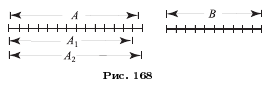
\includegraphics{mppics/ris-168}
\caption{}\label{1938/ris-168}
\end{figure}

Пусть, например, надо измерить отрезок $a$ (рис.~\ref{1938/ris-168}) при помощи единицы $b$.
Тогда поступают так:
положим, что мы желаем найти отрезки, которые отличались бы от $a$ меньше, чем на
$\tfrac1{10}$ единицы длины $b$.
Тогда делим единицу $b$ на 10 равных частей (рис.~\ref{1938/ris-168}) и одну такую долю откладываем на отрезке $a$ столько раз, сколько возможно.
Пусть она уложится 13 раз с некоторым остатком меньшим $\tfrac1{10}b$.
Тогда получим отрезок $a_1=\tfrac{13}{10}b$ и меньший, чем~$a$.
Отложив $\tfrac1{10}b$ ещё один раз, получим другой отрезок, $a_2=\tfrac{14}{10}b$,  больший, чем $a$, который разнится от $a$ менее чем на $\tfrac1{10}$ единицы.
Длины отрезков $a_1$ и $a_2$ выражаются числами $\tfrac{13}{10}$ и $\tfrac{14}{10}$.
Эти числа рассматриваются как \so{приближённые меры} длины отрезка $a$:
первое с недостатком, второе — с избытком.
При этом, так как отрезок $a$ разнится от $a_1$ и от $a_2$ менее чем на $\tfrac1{10}$ единицы, то принято говорить, что каждое из этих чисел выражает длину отрезка $a$ с точностью до $\tfrac1{10}$.

Вообще, чтобы найти приближённые меры длины отрезка $a$ с точностью до $\tfrac1n$ единицы, делят единицу $b$ на $n$ равных частей и узнают, сколько раз $\tfrac1n$-я доля единицы содержится в $a$;
если она содержится $m$ раз с некоторым остатком, меньшим $\tfrac1n b$, то числа $\tfrac mn$ и $\tfrac {m+1}n$ считаются приближёнными мерами длины отрезка $a$ с точностью до $\tfrac1n$-й, первое с недостатком, второе — с избытком.

Может случиться, что этим путём мы найдём точный результат, то есть если отрезок $\tfrac1n b$ уложится целое число раз в отрезке $a$.

Для получения того числа, которое можно было бы принять за точную меру длины отрезка $a$, поступают следующим образом.

Вычисляют последовательно приближённую меру длины отрезка $a$ с недостатком с точностью до $0{,}1$, затем ту же меру с недостатком с точностью до $0{,}01$, затем её же с точностью до $0{,}001$ и продолжают беспредельно этот процесс последовательного вычисления приближённой меры длины $a$, каждый раз повышая точность в 10 раз.
При таком процессе будут получаться последовательно десятичные дроби сначала с одним десятичным знаком, затем с двумя, тремя и дальше всё с б\'{о}льшим и б\'{о}льшим числом десятичных знаков.
Неограниченное продолжение описанного процесса построения десятичных дробей определяет бесконечную десятичную дробь.

Бесконечную десятичную дробь нельзя, конечно, полностью записать на листе бумаги, так как число её десятичных знаков бесконечно.
Тем не менее её считают известной, если известен способ, при помощи которого можно определить любое число её десятичных знаков.


\paragraph{Бесконечные десятичные дроби.}\label{1938/151}
Введение бесконечных десятичных дробей производится в алгебре на основе следующих определений.

1) Бесконечная десятичная дробь называется вещественным числом.

2) Две бесконечные десятичные дроби считаются равными, если их десятичные знаки одинакового порядка равны.

3) Из двух неравных бесконечных десятичных дробей считается б\'{о}льшим вещественным числом та дробь, в которой первый из неравных десятичных знаков одинакового порядка со второй дробью больше.

4) Если в бесконечной десятичной дроби все десятичные знаки, начиная с некоторого порядка, равны нулю, то дробь считается равной той конечной десятичной дроби, которая получится из данной зачёркиванием всех нулей, стоящих справа от последней значащей цифры.
Так, бесконечная десятичная дробь $7{,}8530078000\dots$
равна конечной дроби $7{,}8530078$.

5) Бесконечная периодическая дробь с периодом 9 всегда заменяется конечной десятичной дробью, получаемой из данной увеличением на единицу её последнего десятичного знака, отличного от $9$, и отбрасыванием всех последующих девяток.
Так, дробь $3{,}72999\dots$ заменяют конечной дробью $3{,}73$.

\paragraph{Приближённые значения бесконечной десятичной дроби.}\label{1938/152}
Если оборвать данную бесконечную десятичную дробь на её $n$-м знаке, то полученная конечная дробь называется приближённым значением бесконечной десятичной дроби с точностью до $\tfrac1{10^n}$ с недостатком.
Если же в этой дроби увеличить на единицу её последний десятичный знак, то есть
прибавить к ней $\tfrac1{10^n}$, то получится новая конечная дробь, которая называется приближённым значением бесконечной дроби с той же точностью с избытком.
Если приближённое значение вещественного числа $\alpha$ с $n$ десятичными знаками с недостатком обозначим через $\alpha_n$, а с избытком через  $\alpha_n'$, то  $\alpha_n'=\alpha_n+\tfrac1{10^n}$.
Из определения неравенства вещественных чисел следует, что 
\[\alpha_n\le \alpha<\alpha_n';\]
то есть приближённое значение взятое с недостатком не превосходит само число,
а само число меньше своего приближённого значения с избытком.

Пусть, например, дано вещественное число, определяющее  $\sqrt{2}  \z= 1{,}414\dots$;
его приближённое значение с точностью до $0{,}01$ с недостатком:
$1{,}41$, с избытком:
$1{,}42$;
так как
\begin{align*}
1{,}41 &= 1{,}41000,
&
1{,}42 &= 1{,}42000.
\end{align*}
то в силу определения неравенства вещественных чисел имеем:
\begin{align*}
 1{,}41000\ldots
&< 1{,}414\ldots
< 1{,}42000\ldots,
\intertext{или}
1{,}41 &<  \sqrt{2}  < 1{,}42.
\end{align*}

\paragraph{Сложение вещественных чисел.}\label{1938/153}

Пусть даны два вещественных числа $\alpha$ и $\beta$.
Возьмём их приближённые значения с произвольным числом $n$ десятичных знаков, сначала с недостатком, а затем с избытком.
Приближённые значения чисел $\alpha$ и $\beta$ с недостатком обозначим соответственно через $\alpha_n$ и $\beta_n$, а приближённые значения с избытком — через $\alpha_n'$ и $\beta_n'$.
При этом:
\[\alpha_n'=\alpha_n +\tfrac1{10^n},
\quad
 \beta_n'=\beta_n +\tfrac1{10^n}.\eqno(1)
\]
Составим теперь суммы $\alpha_n+\beta_n$ и $\alpha_n'+ \beta_n'$.
Каждая из них есть десятичная дробь, содержащая $n$ десятичных знаков.

Назовём первую $\gamma_n$, а вторую $\gamma_n'$:
\[\alpha_n+\beta_n=\gamma_n,\quad\alpha_n'+\beta_n'=\gamma_n'.\]
Складывая почленно равенства (1), получим:
\[\alpha_n'+\beta_n'= \alpha_n + \beta_n + \tfrac2{10^n},\]
или $\gamma_n'=\gamma_n+ \tfrac2{10^n}$.
Это равенство показывает, что дробь $\gamma_n$ получается из
дроби $\gamma_n$ прибавлением двух единиц к её последнему десятичному знаку.

Будем теперь увеличивать $n$;
в таком случае дробь $\gamma_n$ приведёт к образованию бесконечной десятичной дроби, которую обозначим~$\gamma$.
Эта дробь может оказаться или периодической, или непериодической.

Допустим, что дробь $\gamma$ непериодическая.
В таком случае она должна содержать бесчисленное множество десятичных знаков, отличных от 9.
В этом случае в дроби $\gamma$ число десятичных знаков, отличных от 9, должно возрастать с возрастанием $n$.
Так как прибавка в дроби $\gamma$ числа $\tfrac2{10^n}$ не может оказать влияния на её десятичные знаки, стоящие левее двух последних знаков, отличных от 9, то число общих первых десятичных знаков в дробях $\gamma_n$ и $\gamma_n'$ будет неограниченно возрастать с возрастанием $n$.
Следовательно, дробь $\gamma_n'$ будет приводить к той же бесконечной десятичной дроби, что и дробь $\gamma_n$.
При этом из предыдущего следует, что при любом~$n$
\[\gamma_n\le \gamma<\gamma_n'.\eqno(2)\]

Допустим теперь, что дробь $\gamma$ периодическая.
В таком случае она представляет собой некоторое рациональное число.
Это число и только оно удовлетворяет неравенству (2) при всех $n$. 

\smallskip
\so{Определение}.
\emph{Вещественное число $\gamma$, удовлетворяющее неравенствам (2) при всех $n$, называется суммой вещественных чисел $\alpha$ и $\beta$.}
\[\gamma=\alpha+\beta.\]

\paragraph{Другие действия с вещественными числами.}\label{1938/154}
Совершенно аналогичным образом можно определить разность двух вещественных чисел, их произведение и частное от деления одного вещественного числа на другое.
Более подробное изучение результатов этих действий показывает, что определённые таким образом сумма и произведение вещественных чисел подчиняются основным законам действий, имеющим место для чисел рациональных:
сложение подчиняется переместительному и сочетательному законам.

\[\alpha+\beta=\beta+\alpha,
\quad
(\alpha+\beta)+\gamma=\alpha+(\beta+\gamma),
\]
а умножение — переместительному, сочетательному и распределительному законам.
\[\alpha\beta=\beta\alpha,
\quad
(\alpha\beta)\gamma=\alpha(\beta\gamma),
\quad
(\alpha+\beta)\gamma=\alpha\gamma+\beta\gamma.
\]

В тех случаях, когда бесконечные десятичные дроби будут периодическими, определённые выше действия над ними будут приводить, как легко показать, к тем же результатам, что и действия над обыкновенными дробями, получаемыми после обращения периодических дробей в простые.

Таким образом, рациональные числа являются лишь частным видом вещественных чисел.
 
\paragraph{Длины отрезков и их отношения.}\label{1938/155}
Число, получаемое в результате измерения отрезка $a$, называется \rindex{длина}\textbf{длиной} этого отрезка.

Заметим, что равенство длин отрезков и равенство отрезков, определённое нами с помощью наложения (§~\ref{1938/6}), эквивалентны, конечно, если для измерения отрезков мы пользовались одной единицей длины.
То же верно и для сравнения, сложения и других действий над отрезками и их длинами (§§~\ref{1938/6}—\ref{1938/8}).

Например неравенство $AB>2\cdot CD$ может пониматься двояко — то что отрезок $CD$ укладывается два раза в отрезке $AB$ с некоторым остатком и то, что длина отрезка $AB$ больше чем удвоенная длина отрезка $CD$ измеренная той же единицей длины.
При этом выражение «измеренная той же единицей длины» мы будем опускать, предполагая что
в каждой конкретной задаче, измерения производятся только одной единицей.

Под отношением двух отрезков мы понимаем отношение их длин. 
Это же отношение равно длине первого если второй взять за единицу длины.

Заметим, что отношение двух отрезков не зависит от того, как выбрана единица измерения.
В самом деле, если, например, вместо одной уже выбранной единицы измерения взять другую, в 3 раза меньшую, то в каждом отрезке эта новая единица уложится втрое большее число раз, чем прежняя.
В той дроби, которая представляет отношение отрезков, числитель и знаменатель оба увеличатся в 3 раза.
Величина же самой дроби от этого не изменится.

\paragraph{Пропорции.}\label{extra/proportions}
В геометрических задачах часто появляется уравнение типа  
\[\frac{a}{b}=\frac{c}{d}\eqno(1)\]
на длины $a$, $b$, $c$ и $d$ некоторых отрезков.
Такое уравнение называется \rindex{пропорция}\textbf{пропорцией}. 

Следующие наблюдения часто оказываются полезными:

1) Пропорцию (1) можно переписать как произведение:
\begin{align*}
a\cdot d&=b\cdot c.
\end{align*}

2) Пропорцию (1) можно продолжить складывая или вычитая соответствующие члены: 
\[\frac{a}{b}=\frac{c}{d}=\frac{a+c}{b+d}=\frac{a-c}{b-d}=\frac{2a+3c}{2b+3d}=\dots\]
конечно если знаменатели в новых дробях не равны нулю.

3) По пропорции (1) можно написать другие пропорции, например:
\begin{align*}
\frac{a}{c}&=\frac{b}{d},
\\
\frac{a+b}{b}&=\frac{b+c}{b},
\\
\frac{a}{b-a}&=\frac{c}{d-c}\quad \text{и так далее.}
\end{align*}

Приведём пример использования этих наблюдений.

\smallskip
\so{Задача 1}. Предположим для точек $C$ и $C'$ лежащих на отрезке $AB$ выполняется пропорция
\[\frac{AC}{CB}=\frac{AC'}{C'B}.\eqno(2)\]
Доказать, что $C=C'$.

Из пропорции (2) можно написать другую
\[\frac{AC}{AC+CB}=\frac{AC'}{AC'+C'B}.\]
Поскольку точки $C$ и $C'$ лежат на отрезке $AB$, 
\[AC+CB=AC'+C'B=AB.\]
Значит
\[\frac{AC}{AB}=\frac{AC'}{AB};\]
следовательно $AC=AC'$ и $C=C'$.

Аналогично решается следующая задача:

\smallskip
\so{Задача 2}. Предположим для точек $C$ и $C'$ лежащих на продолжении отрезка $AB$ выполняется пропорция
\[\frac{AC}{CB}=\frac{AC'}{C'B}.\eqno(3)\]
Доказать, что $C=C'$.

Не умоляя общности можно предположить, что $AC>CB$;
тогда из пропорции (3) следует, что $AC'>C'B$,
то есть обе точки $C$ и $C'$ лежат на продолжении $AB$ за точку $B$ и значит 
\[AC-CB=AC'-C'B=AB.\]
Из пропорции (3) можно написать другую
\[\frac{AC}{AC-CB}=\frac{AC'}{AC'-C'B}\]
или
\[\frac{AC}{AB}=\frac{AC'}{AB};\]
следовательно $AC=AC'$ и $C=C'$.
